\section{H-bro - Motorstyring} \label{sec:hwi_motor_driver}
\subsection*{Ultiboard}

Efter at have designet motorstyrings kredsløbet fra figur \ref{fig:MultiSim_HBro} på side \pageref{fig:MultiSim_HBro} i MultiSim bliver det overført til Ultiboard. Her er printet lagt ud med henblik på at reducerer EMC støj fra printet. Printet er delt op i 2 dele. Et med signaler fra PI på 3,3 V ydeste til højre på figur \ref{fig:Ultiboard_Print_H_Bro}. Et til 5V til det logiske kreds på L298N og 7,2V til motor forsyning. De 2 sidste er så vidt muligt holdt væk fra signaler fra PIen. De baner til 7,2V motor forsyning til og fra L298N er gjort så korte som muligt og tæt på returbaner. Så der undgås store strømloops der kan lave en masse EMC støj. Der er desuden lavet et ground plane der også er med til at reducere EMC støj.

\begin{figure}[h]
	\centering
	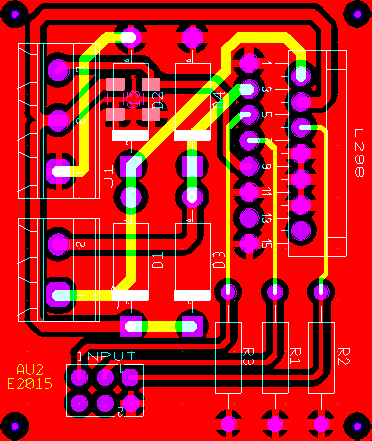
\includegraphics[width=\textwidth* 4/10, angle =90]{../fig/billeder/Ultiboard_H_Bro}
	\label{fig:Ultiboard_H_Bro}
	\caption{Ultiboard H-Bro}
\end{figure}

\begin{figure}[h]
	\centering
	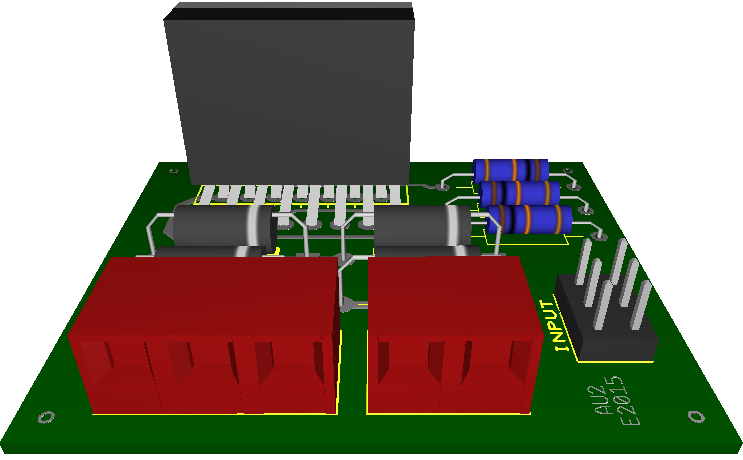
\includegraphics[width=\textwidth* 5/10]{../fig/billeder/Ultiboard_Print_H_Bro}
	\label{fig:Ultiboard_Print_H_Bro}
	\caption{Ultiboard 3D view af print for H-Bro}
\end{figure}

\clearpage
\subsection*{Færdig print}



\begin{figure}[h]
	\centering
	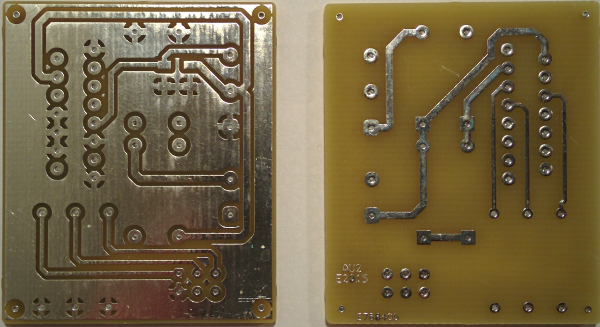
\includegraphics[width=\textwidth* 7/10]{../fig/billeder/Ultiboard_Print_Bare}
	\label{fig:Ultiboard_Print_H_Bro_Bare}
	\caption{Print for H-Bro før komponenter monteret}
\end{figure}

\begin{figure}[h]
	\centering
	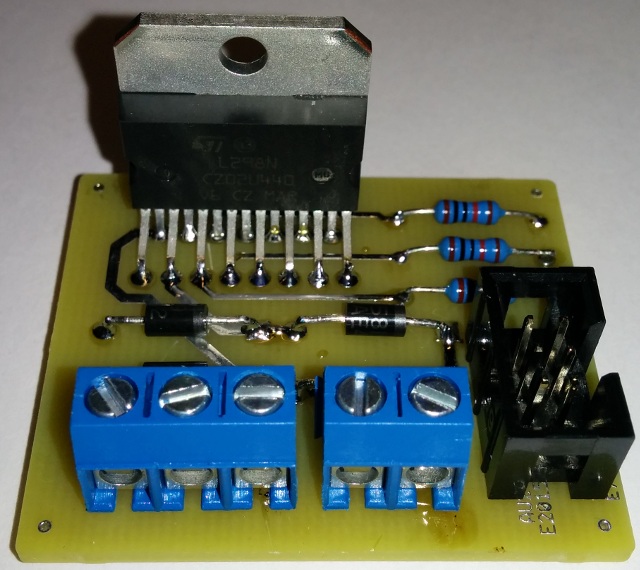
\includegraphics[width=\textwidth* 5/10]{../fig/billeder/Print_H_Bro}
	\label{fig:Print_H_Bro_finished}
	\caption{Print for H-Bro med komponenter monteret}
\end{figure}

\subsection{Test}

For at test H-broen blev printet først testet med en funktionsgenerator og oscilloskop. Da det så ud til at virke efter hensigten blev den sat til bilens motor. Og til sidst blev funktionsgenerator udskiftet med Pi'en med et PWM test program.
\clearpage